\documentclass{article}
\usepackage[utf8]{inputenc}
\usepackage{natbib}
\usepackage{graphicx}
\usepackage{indentfirst}
\usepackage{enumitem}
\usepackage{amssymb}
\usepackage{amsmath}
\usepackage{float}
\usepackage{listings}
\usepackage{color} %red, green, blue, yellow, cyan, magenta, black, white
\definecolor{mygreen}{RGB}{28,172,0} % color values Red, Green, Blue
\definecolor{mylilas}{RGB}{170,55,241}


\title{Project 2}
\author{Matthew Callahan, Jiajing Guan, and Aneesh Malhotra}
\date{October 22, 2018}

\begin{document}

\maketitle
\section{Trajectory Matching with Markov Chain Monte Carlo}
\subsection{Method}
Since the ODE function given could be easily solved, the problem became estimating $C$ and $\beta$ in $Ce^{-\beta t}$.\\
We first initialized the Markov Chain Monte Carlo with the following parameters:\\
\begin{center}
\begin{tabular}{|c|c|}
\hline
Variable & Value\\
\hline
$C_0$ & 0\\
$\beta_0$ & 0\\
Data Standard Deviation $\sigma$ & 0.03\\
Guess Jump & 0.01\\
Burn Time & 100\\
Iteration Limit & 5000\\
\hline
\end{tabular}
\end{center}
For each iteration step, we make a new guess for $[C_n,\beta_n]=[C_{n-1},\beta_{n-1}]+D*\text{randn}$. Then we calculate the SSE using $[C_n,\beta_n]$ to evaluate the ratio $e^{\frac{-\text{SSE}_{n-1}+\text{SSE}_n}{2\sigma^2}}$. If a random number between 0 and 1 is smaller than the ratio, the new guess is accepted. \\
\subsection{Result}
Using the method described above, we obtained the estimated parameters on two sets of data given.
\begin{itemize}
\item Smooth Data
With the smoother version of the data, we obtained the following result:
\begin{center}
\begin{tabular}{|cc|}
\hline
C & 3.1792\\
\hline
$\beta$ & 5.5447\\
\hline
\end{tabular}
\end{center}
\pagebreak
We can also observe the convergence in the following figure:
\begin{figure}[H]
\centering
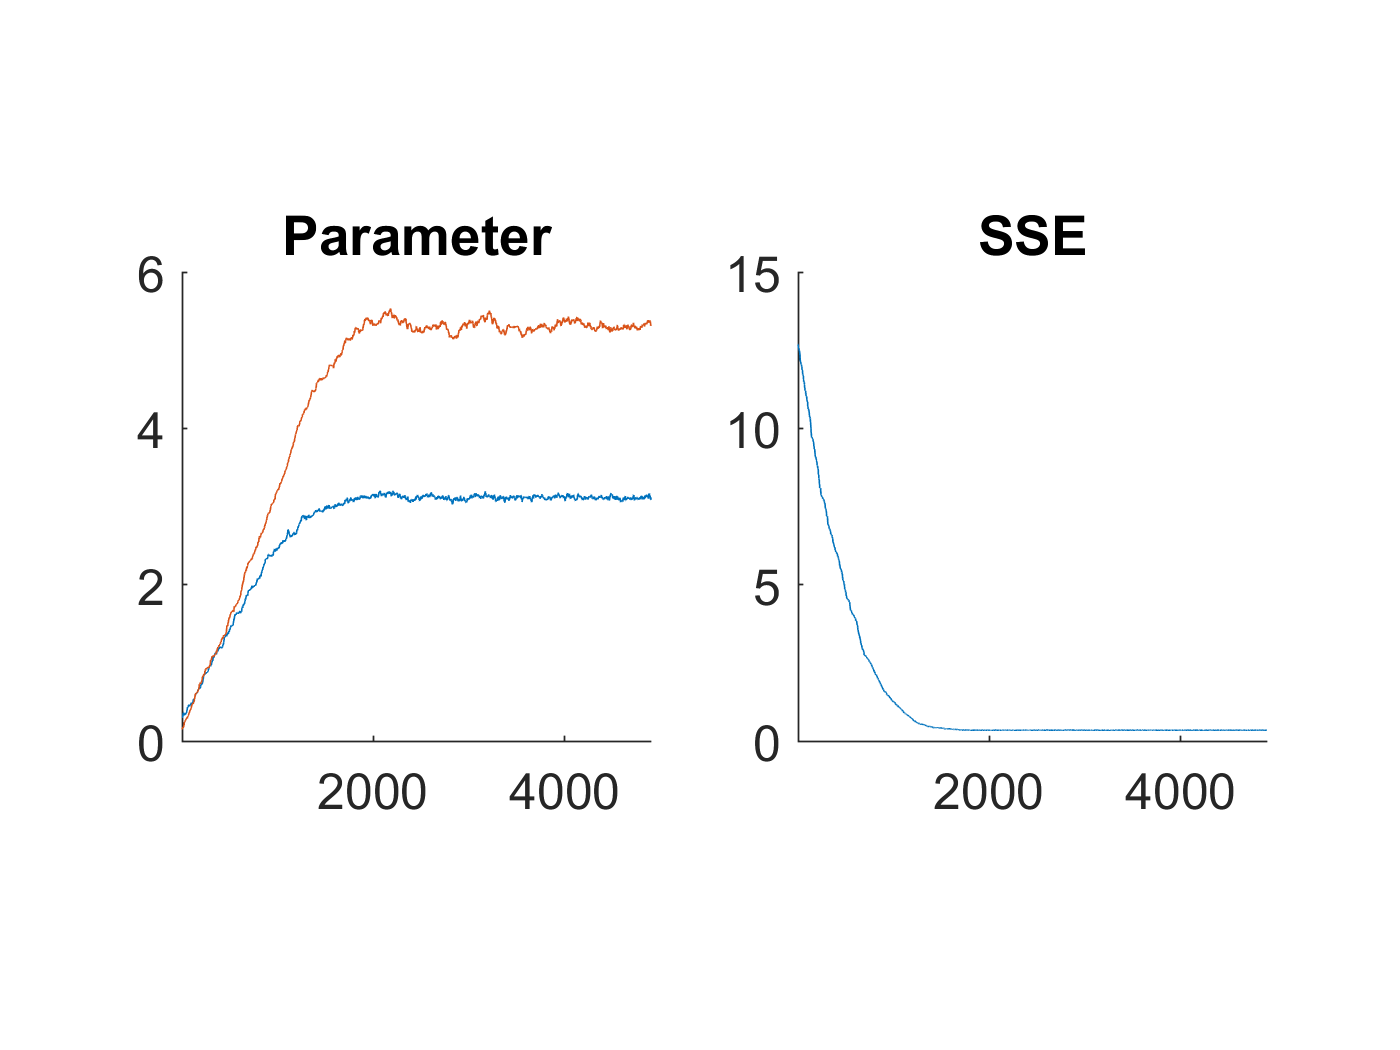
\includegraphics[scale=0.3]{figures/p_a_conv.png}
\caption{The figure on the left shows the convergence of the parameters as iteration step increases. The figure on the right shows the convergence of SSE.}
\end{figure}

We can also see how our model compares with the data:
\begin{figure}[H]
\centering
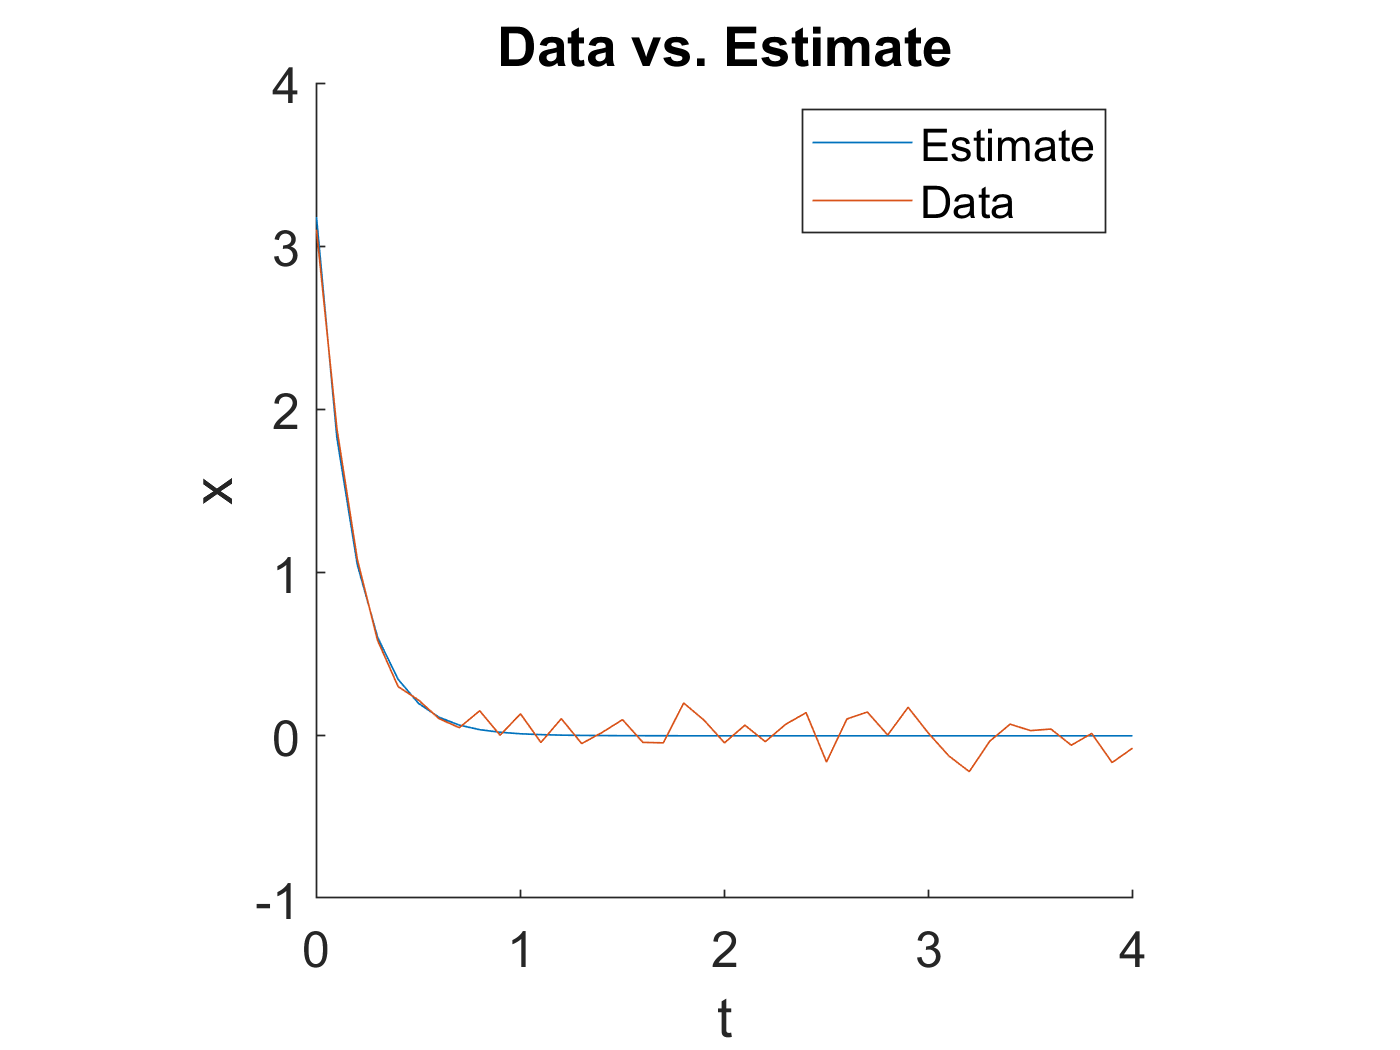
\includegraphics[scale=0.2]{figures/p_a_data.png}
\caption{The model we obtained is the line in blue. We can see that our model captures the trend of the data.}
\end{figure}

\item Noisy Data

With the noisy version of the data, we obtained the following result:
\begin{center}
\begin{tabular}{|c|c|}
\hline
C & 2.6331\\
\hline
$\beta$ & 4.8364\\
\hline
\end{tabular}
\end{center}

We can also observe the convergence in the following figure:
\begin{figure}[H]
\centering
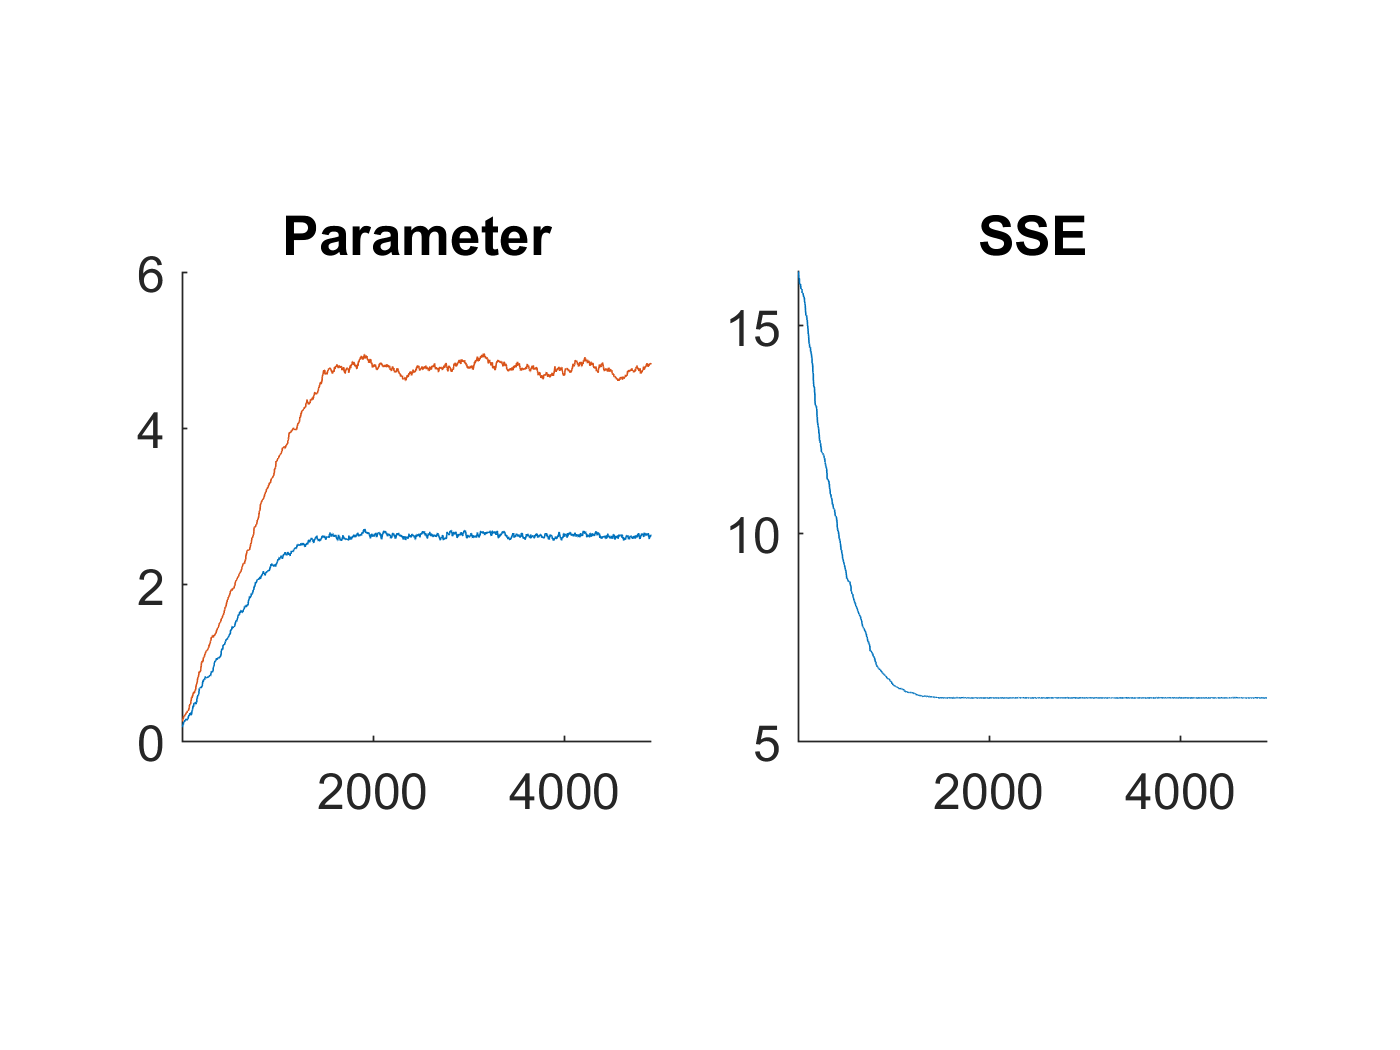
\includegraphics[scale=0.3]{figures/p_a_conv_1.png}
\caption{The figure on the left shows the convergence of the parameters as iteration step increases. The figure on the right shows the convergence of SSE.}
\end{figure}

We can also see how our model compares with the data:
\begin{figure}[H]
\centering
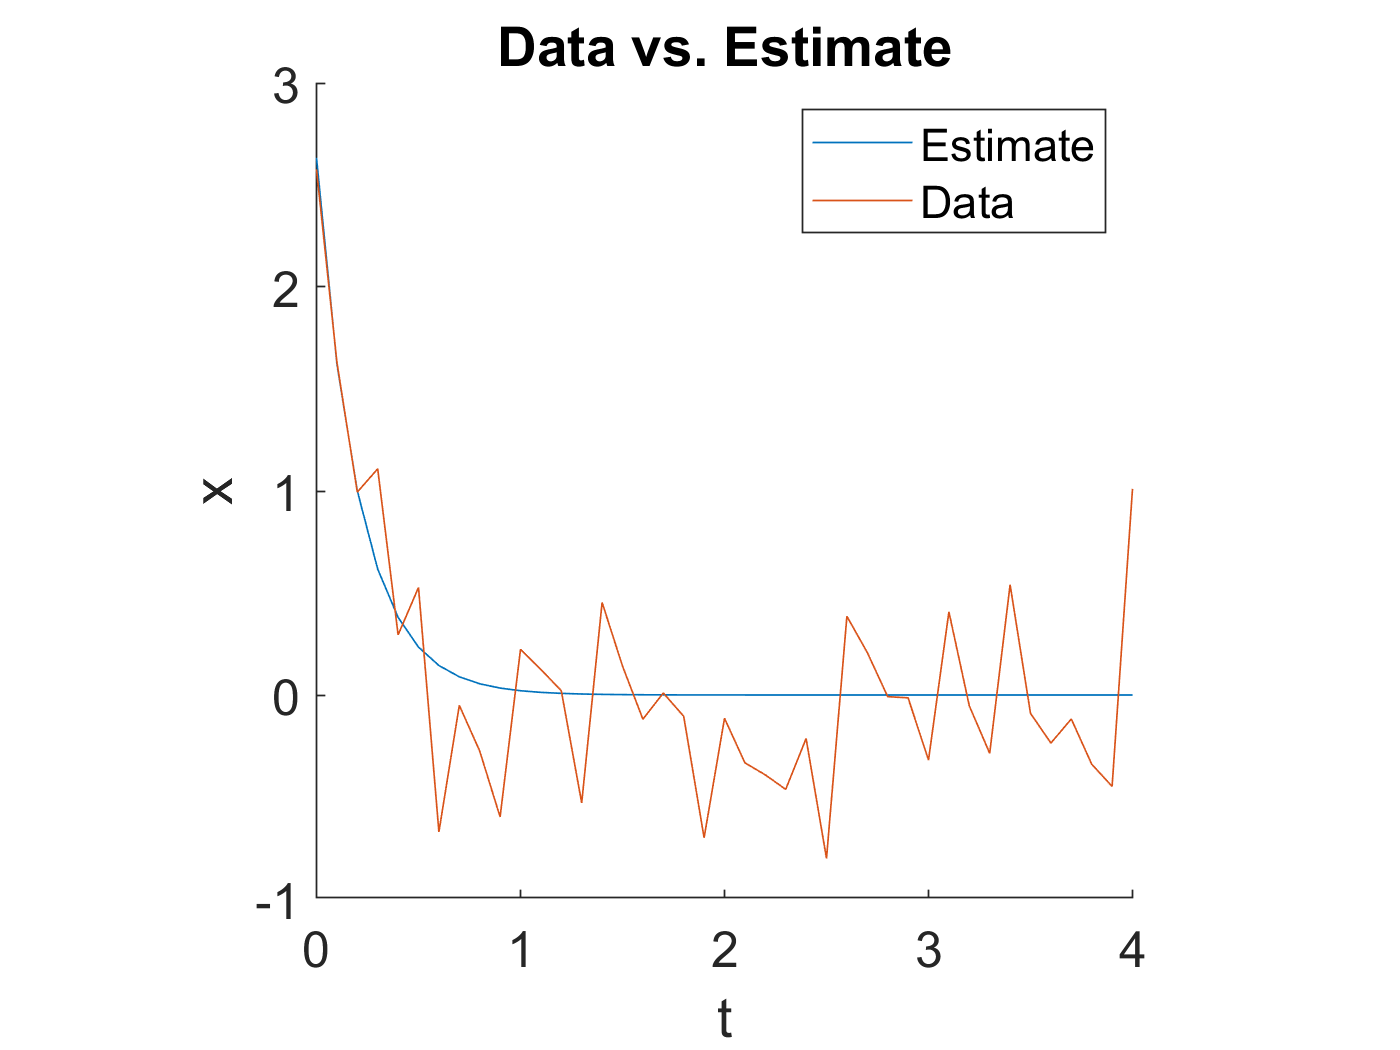
\includegraphics[scale=0.2]{figures/p_a_data_1.png}
\caption{The model we obtained is the line in blue. We can see that our model captures the trend of the data.}
\end{figure}
\end{itemize}

\subsection{Explore}
We explored with the guess jump a little bit and obtained the following result:
\begin{center}
\begin{tabular}{|c|c|c|c|c|}
\hline
Guess Jump & C & $\beta$ & Convergence Step& Converged SSE\\
\hline
0.005 & 3.16566068356473 & 5.46532123092112 & 4326 & 0.346611467385126\\
0.01 & 3.12005507560874 & 5.35257792035497 & 2073	 & 0.344644620650210\\
0.02 & 3.09761701625579 & 5.27931484301583 & 755 & 0.345845653405011\\
0.1 & 3.17838628697765 & 5.50513291919420 & 99 & 0.348208384804511\\
\hline
\end{tabular}
\end{center}

We can see that the different guess jump did not affect the results too much but did delay convergence when it is small.\\

\section{Gradient Matching with Smoothing}
\subsection{Method}
We can smooth the data using collocation. The basis $\phi$ could be created using \textit{spcol} function in matlab. Then the coefficients $\mathbf{c}=(\phi^{T}\phi)^{-1}(\phi y)$, where $y$ is the data given.\\

The gradient matching method is essentially using Gauss-Newton method to minimize the integrated SSE:
$$\text{ISSE}=\sum_{i=1}^n W_{i} [D\hat{x(t_i)}-f(\hat{x(t_i)},\theta)]^2$$
where $\hat{x(t_i)}=\phi \mathbf{c}$ is the smoothed data using collocation. \\
For this problem, the ISSE could be simplied to 
$$\text{ISSE}=\sum_{i=1}^n W_{i} [D\phi(t_i)\mathbf{c}+\beta \phi(t_i)\mathbf{c}]^2$$
Then the Jacobian becomes $\hat{x}$. For each iteration step, we perform the following:
\begin{center}
\begin{equation}
\begin{split}
H & = J^{T}J\\
g & = J^{T}(D\hat{x}+\beta\hat{x})\\
\beta_n & = \beta_{n-1} - H^{-1}g
\end{split}
\end{equation}
\end{center}
Due to the fact that ISSE does not take $x(t_0)$ into account, we use the initial value of the smoothed data as $x(t_0)$ for the following parts.

\subsection{Result}
\begin{itemize}
\item Smooth Data
The estimated $\beta=4.962410410929266$.\\
We can also observe the convergence in the following figure:
\begin{figure}[H]
\centering
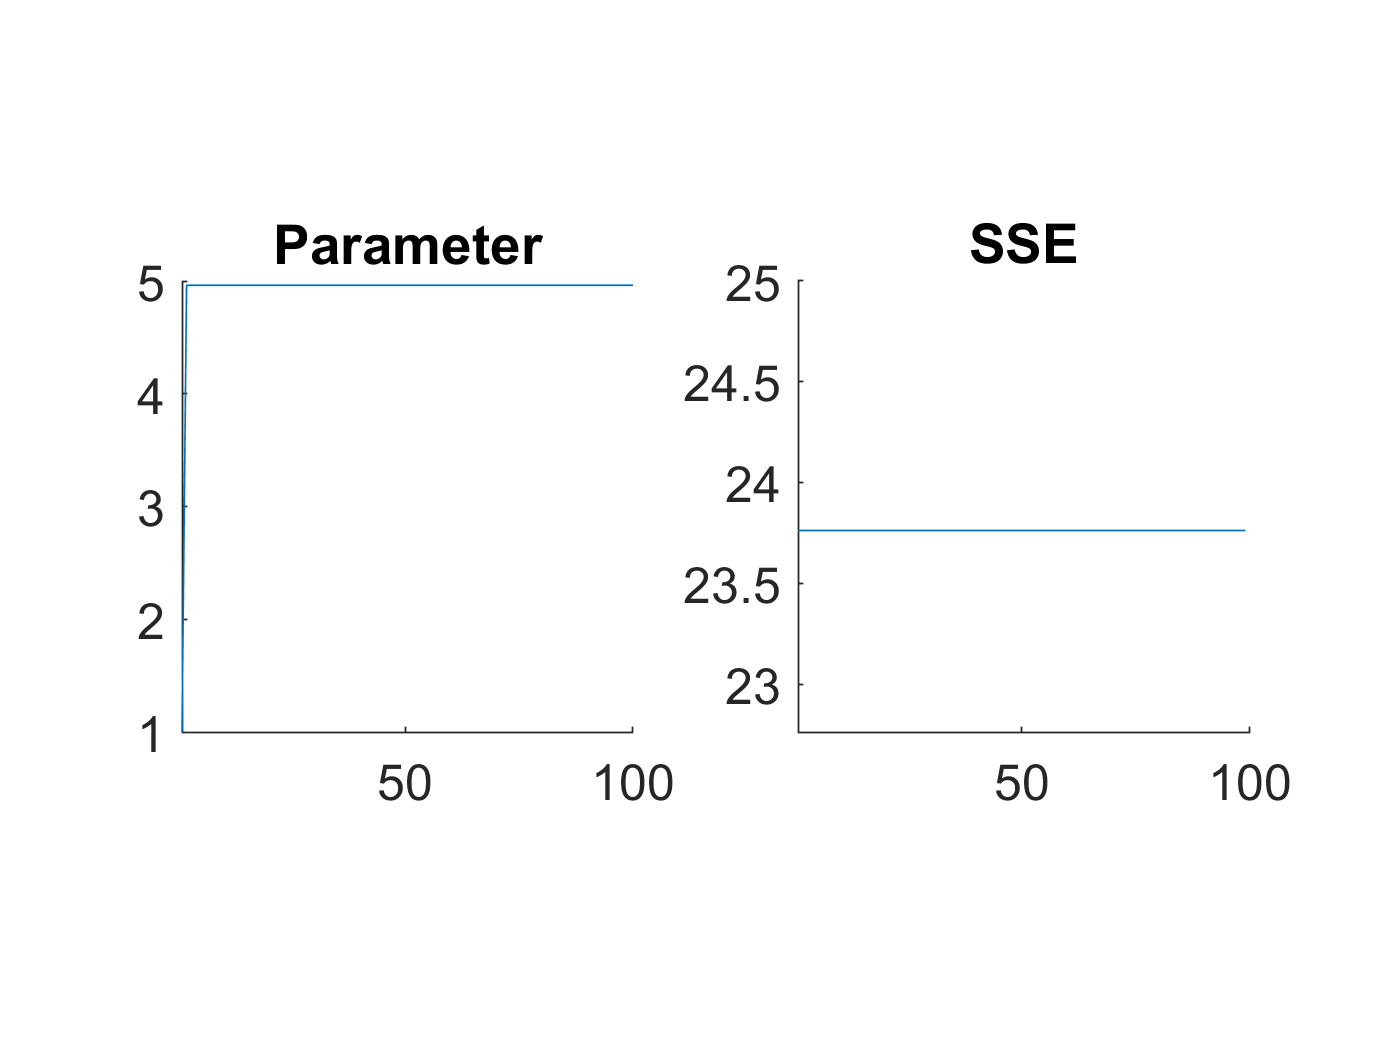
\includegraphics[scale=0.3]{figures/p_b_conv.png}
\caption{The figure on the left shows the convergence of the parameters as iteration step increases. The figure on the right shows the convergence of SSE.}
\end{figure}

We can also see how our model compares with the data:
\begin{figure}[H]
\centering
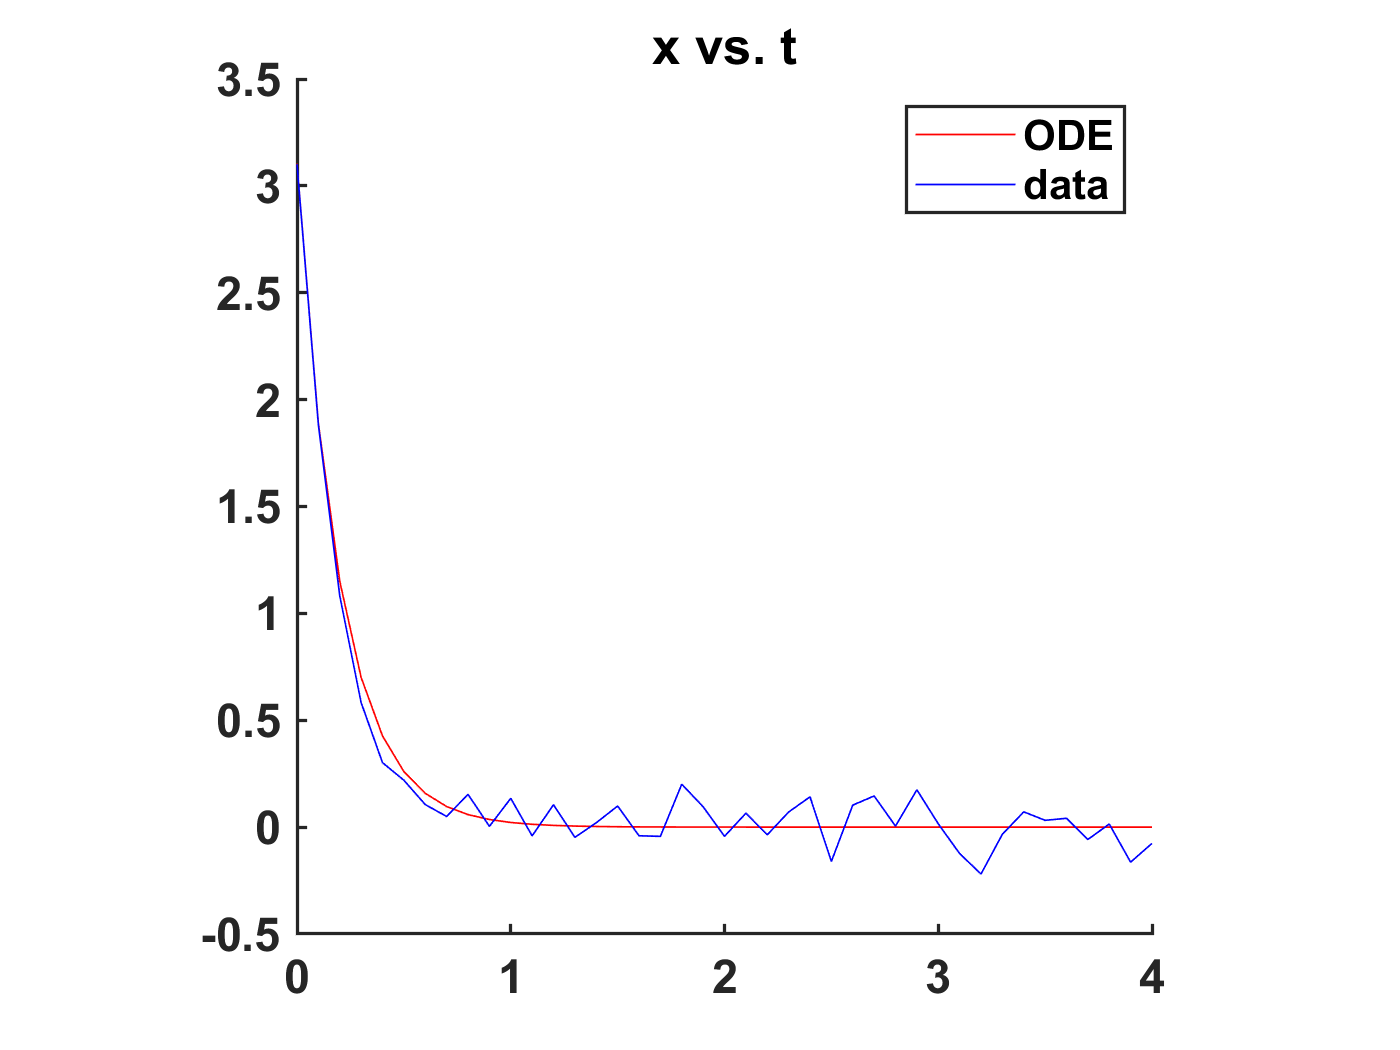
\includegraphics[scale=0.2]{figures/p_b_data.png}
\caption{The model we obtained is the line in blue. We can see that our model captures the trend of the data.}
\end{figure}

\item Noisy Data
The estimated $\beta=2.160787567688269$.\\
We can also observe the convergence in the following figure:
\begin{figure}[H]
\centering
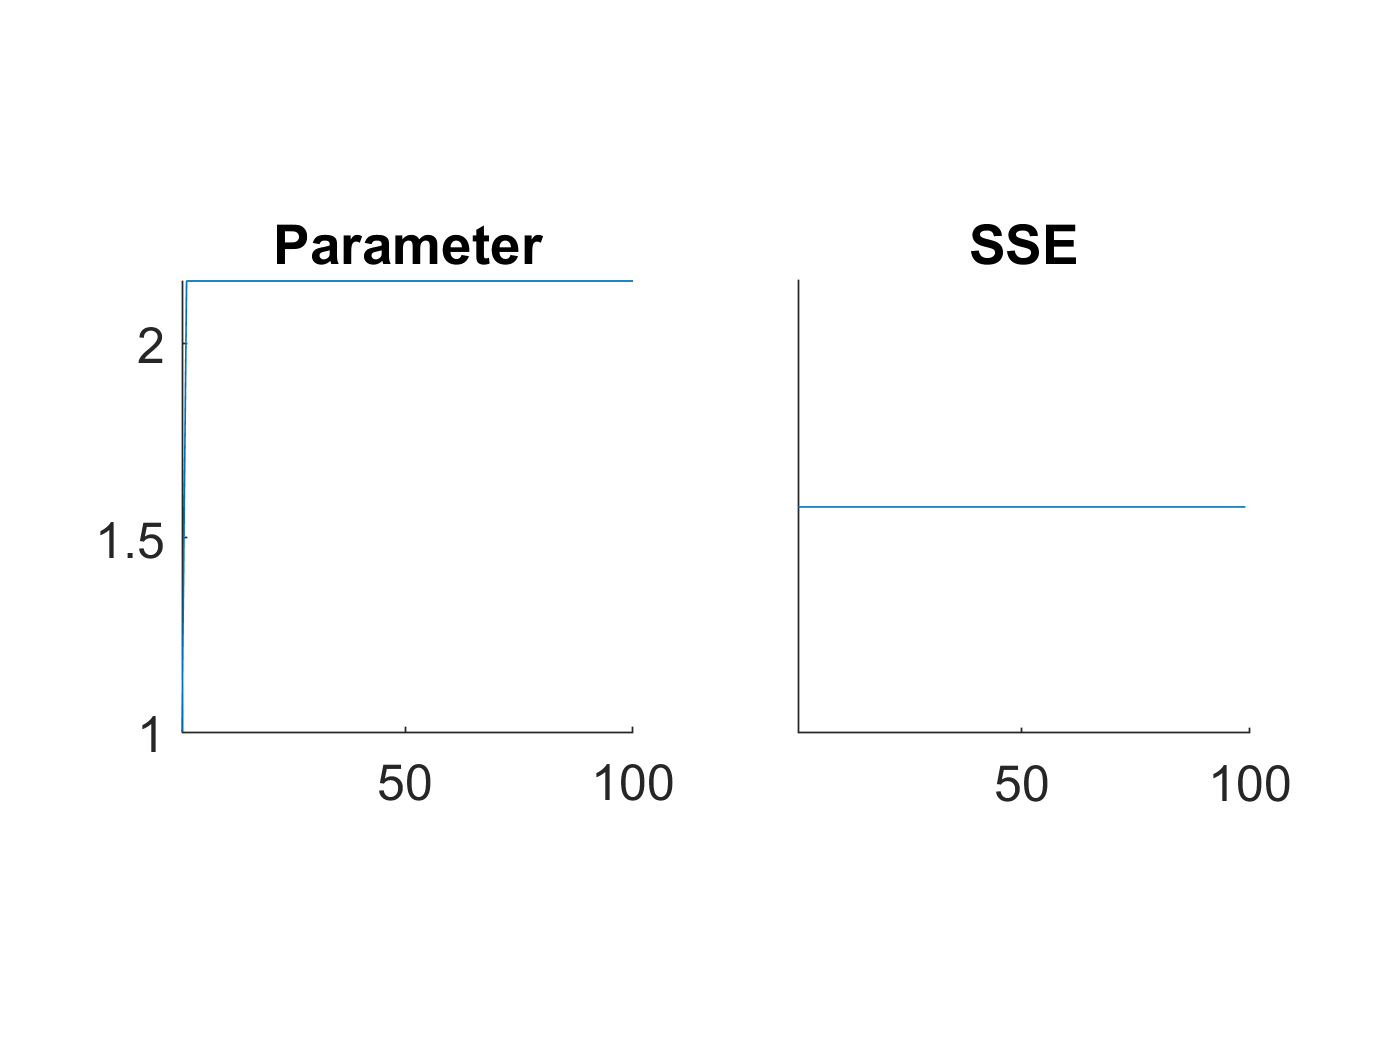
\includegraphics[scale=0.3]{figures/p_b_conv_1.png}
\caption{The figure on the left shows the convergence of the parameters as iteration step increases. The figure on the right shows the convergence of SSE.}
\end{figure}

We can also see how our model compares with the data:
\begin{figure}[H]
\centering
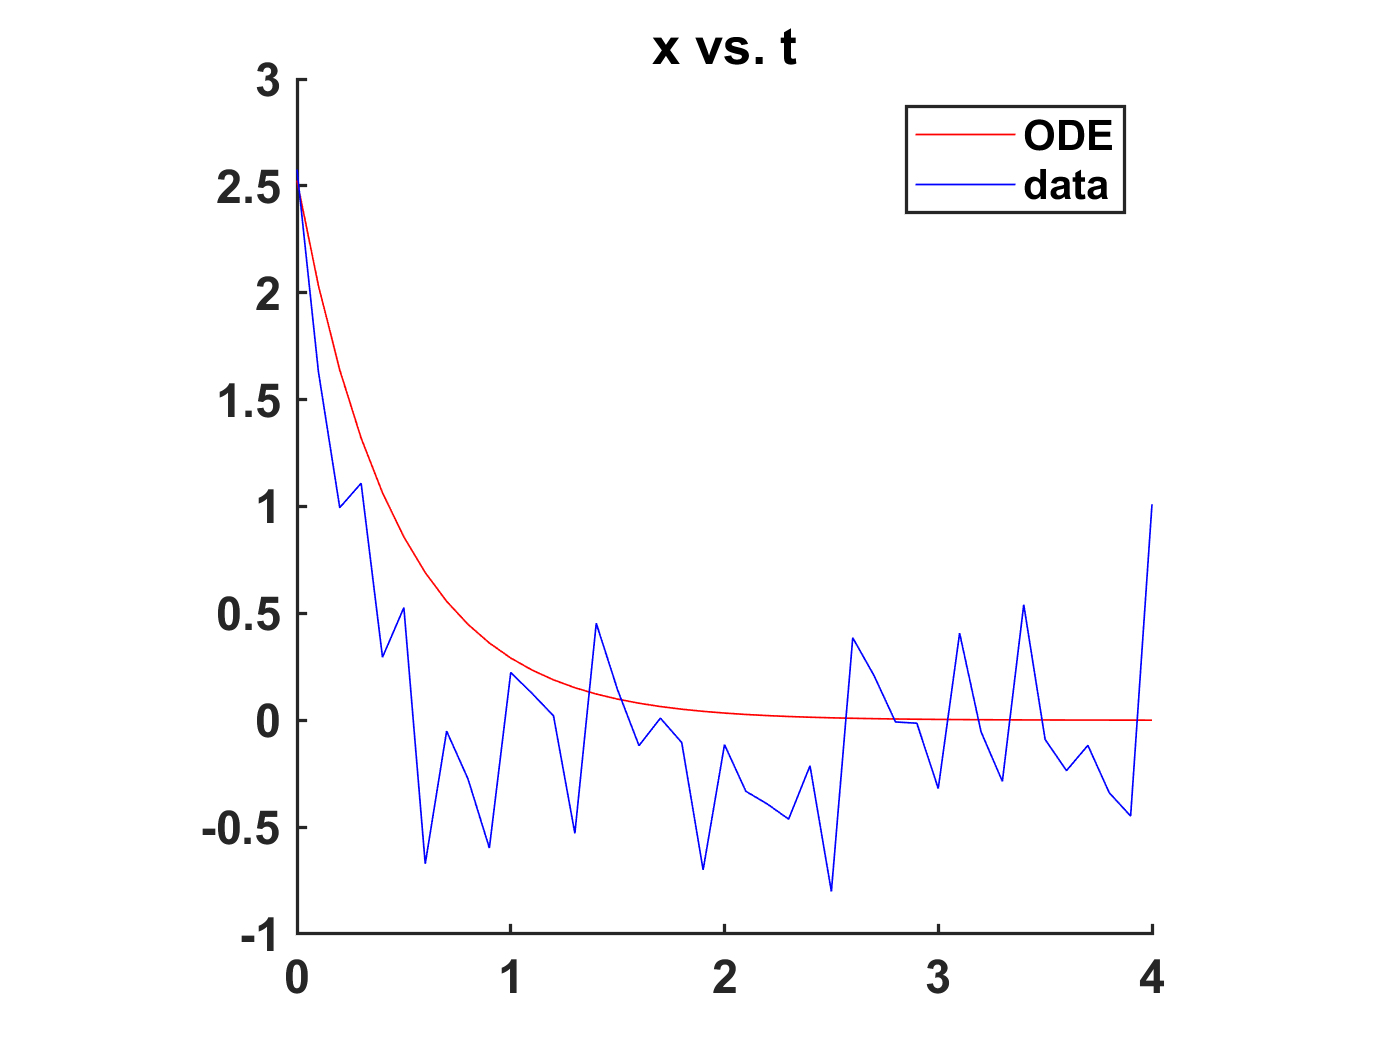
\includegraphics[scale=0.2]{figures/p_b_data_1.png}
\caption{The model we obtained is the line in blue. We can see that our model captures the trend of the data.}
\end{figure}

\end{itemize}
\subsection{Explore}
\begin{itemize}
\item Without Smoothing\\
When the method is used without smoothing, it fails catastrophically. The parameter blows up.
\item Different Number of Basis\\
When we smooth the data with collocations, we try different number of polynomials allowed for the basis and obtained the following result:\\
\begin{center}
\begin{tabular}{|c|c|}
\hline
Number of Polynomials & $\beta$\\
\hline
9 & 4.97277486579170\\
10 & 4.94682728787471\\
11 & 4.96241041092927\\
12 & 4.96995381483431\\
13 & 4.97336941885107\\
\hline
\end{tabular}
\end{center}
Therefore, the number of polynomials in the collocation basis does not affect the results drastically. 
\end{itemize}
\section{Integral Matching with Smoothing}
\section{Parameter Cascading with Smoothing}
\section{Comparison}
First, we think that the gradient descent method is most helpful when the initial value does not to be  approximated. Otherwise, it limits the accuracy of the model.\\\\
Second, we think that the MCMC and integral matching method are powerful when the ODE equations given can be easily solved. The MCMC method is easier than the integral matching method because we don't need to take the Jacobian matrix.\\\\
Profile cascading method required the most time coding in all of these methods, but the method is overall more powerful than others. It converges fast and provides accurate estimation for the parameters.
\end{document}
